\section{Extraction de termes avec Word2Vec}
Nous avons entraîné un modèle Word2Vec sur un corpus de comptes rendus de maintenance sur des éoliennes. Ce corpus contient XXXX fiches de maintenance pour une volumétrie de XXXX Mo. Si la taille de ce corpus semble restreinte, nous avons néanmoins obtenu des résultats concluants (fig \ref{fig:w2v}), les textes étant très répétitifs (taille de dictionnaire d'environ 5000 mots). Ajout de l'indice de diversité lexicale.

\begin{figure}[tb]
    \begin{center}
        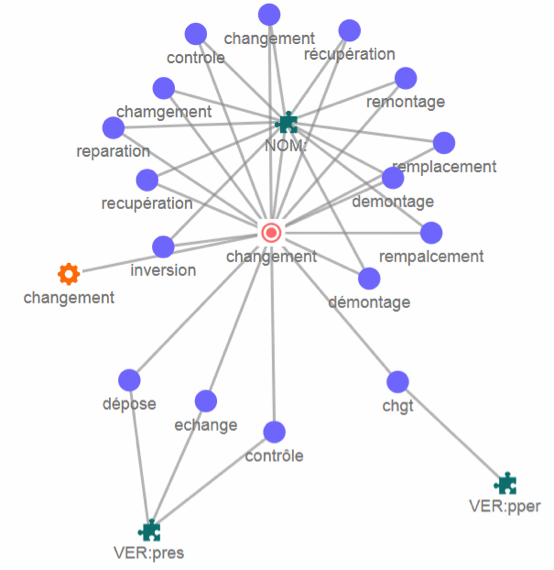
\includegraphics[width=6cm]{figures/w2v}
    \end{center}
    \caption{Visualisation des résultats de Word2Vec}\label{fig:w2v}
\end{figure}

Vérifier algo
Nous avons mis en place un script python qui effectue plusieurs opérations :
\begin{enumerate}

\item Prétraitements : suppressions des caractères non désirés.
\item Découpage en phrases et en mots.
\item Nettoyage des mots : suppression des mots vides.
\item Appel de TreeTagger \cite{Schmid94probabilisticpart-of-speech} pour un étiquetage morphosyntaxique : nous sommes partis de l'hypothèse que l'apprentissage de Word2Vec serait plus fin avec l'ajout de métadonnées de type morphosyntaxique sur les mots de notre corpus. Word2vec apprend sur la forme, le lemme et la catégorie morphosyntaxique du terme. Nous considérons qu'il s'agit d'une première étape de désambiguïsation.
\item Appel du package gensim en python pour le calcul de la similarité avec Word2Vec.
\item Création d'une sortie contenant les résultats de Word2Vec au format RDF.

\end{enumerate}
